\cotefile{145}

\scanpage{3}
Les autom. \inserted{à lacets} de $\hat\Pi_{0,3}=\pi$ commutant \deleted{\unsure{à}} $\sigma_0$, et commutant extérieurement à $\rho$, sont donnés par
\[
u(l_{\unsure{1|0}})=\operatorname{int}(g_1)l_1^{p}
\]
\[
u(l_\infty)=\operatorname{int}(\underbrace{\sigma_0(g_1)}_{g_\infty})l_\infty^{p}
\]
\margin{\uline{NB} on aura
\[
u(l_0)=\operatorname{int}\bigl(\underbrace{g_1l_1^{-\gamma}\rho^{-1}(h_1)}_{g_0}\bigr)\cdot l_0^{p}
\]}
avec $g_1\in\Pi\bmod L_1$, $p\in\hat{\mathbb Z}^{*}$ satisfaisant la condition (où $\beta,\gamma\in\hat{\mathbb Z}$ sont uniquement déterminés par $g_1,p$)
\margin{\uline{et $\bar m$ pas} \uline{$u$}!}
\[
(1)\qquad\boxed{l_\infty^{p}\cdot\operatorname{int}(h_1)(l_1^{p})\cdot\operatorname{int}\bigl(h_1l_1^{-\gamma}\rho^{-1}(h_1)\bigr)(l_0^{p})=1}
\]
et
\[
(2)\qquad\boxed{\rho(h_1)(l_\infty^{-\gamma}\unsure{\cdot|=} h_1l_1^{-\gamma})\rho^{-1}(h_1)=l_0^\beta}
\]
\margin{NB. On doit en fait avoir $\unsure{\beta=\gamma|\beta\ne\gamma}$ (passer à $(\Pi_{0,3})_{\mathrm{ab}}$)}
avec
\[
h_1=\unsure{\sigma_0|\sigma_0'|\dot\sigma_0}(g_1)^{-1}g_1
\]
La deuxième relation s'écrit aussi
\[
h_1l_1^{-\gamma}\rho^{-1}(h_1)=l_\infty^\gamma\rho(h_1)^{-1}l_0^{\deleted{\unsure{\gamma|\alpha}}\beta}
\]
et en portant dans la première relation, celle-ci peut se récrire
\figure{\begin{tikzpicture}[baseline]\draw[->] (0,0.7)--(0,0);\draw (-0.1,0.7)--(0.1,0.7);\end{tikzpicture}}
\[
(1')\qquad\boxed{l_\infty^{p}\cdot\unsure{\operatorname{int}(h_1)|\operatorname{int}h_1}(l_1^{p})\cdot\operatorname{int}\bigl(l_\infty^\gamma\rho(h_1)^{-1}\bigr)(l_0^{p})=1}
\]
\uline{NB} Si on change $g_1$ en $g_1'=g_1l_1^\mu$, $h_1$ est remplacé en $h_1'=l_\infty^{-\mu}h_1l_1^\mu$, et la relation $(1')$ donne, en lui appliquant $\operatorname{int}(l_\infty^{-\mu})$ :
\[
l_\infty^{p}\cdot\operatorname{int}(\deleted{\unsure{h_1}}h_1')(l_1^{p})\cdot\operatorname{int}\bigl(\deleted{\unsure{l_1^\mu|h_1}}l_\infty^{\unsure{\gamma'|\gamma-\mu|\gamma}}\unsure{\rho^{\deleted{\unsure{-1}}}|\rho^{-1}|\rho^1|\hat\rho}(h_1')^{-1}\bigr)(l_0^{p})=1
\]
(\uline{i.e.} \uline{$\gamma'=\gamma\deleted{\unsure{+2\mu|+\mu}}$}) et on a la relation correspondante \unsure{à|:} $(2)_2$ avec $\deleted{\unsure{\beta}}\beta'=\beta$.
\mspage{2}

\scanpage{5}
[C]\qquad\textcircled{1}\qquad\mspage{1}

Automorphismes extérieurs du groupe à lacets \deleted{\unsure{P|$\Pi$}} profini $\hat\Pi=\hat\Pi_{0,3}$
\margin{\uline{et structure}\\\uline{d'extensions}\\\uline{de $\mathcal E=\mathcal E_{\unsure{0,3|03}}$}}
\margin{$\unsure{\partial|\delta}$}

On prend la présentation par les générateurs $l_0,l_1,l_\infty$ liés par
\[
l_0l_1l_\infty=1
\]
Un endomorphisme \unsure{de|du} $\Pi_{0,3}$ est donc donné par des éléments $l_0',l_1',l_\infty'$ satisfaisant la $\bar m$ relation --- sauf erreur ce sera un autom. s'ils engendrent $\pi$ (topologiquement).

Soit $\rho$ l'automorphisme défini par la permutation circulaire
\[
\rho(l_0)=l_1,\quad\rho(l_1)=l_\infty,\quad\rho(l_\infty)=l_0
\]
(donc on a $\rho^3=\mathrm{id}$). Considérons aussi la transposition

\deleted{On s'intéresse aux}
\[
\sigma_\infty(l_0)=l_1,\quad\sigma_\infty(l_1)=l_0,\qquad
\sigma_\infty(l_\infty)=(l_1l_0)^{-1}=l_0^{-1}l_1^{-1}
\]
\inserted{$(=\operatorname{int}(\deleted{\unsure{l_0}}l_0^{-1})\cdot l_\infty)$}

on a évidemment $\sigma_\infty^2=\mathrm{id}$. On définit de $\bar m$ $\sigma_0,\sigma_{\unsure{1|\infty}}$ \inserted{(échangeant $l_1$ et $l_{\unsure{\infty|0}}$ resp. $l_\infty$ et $l_0$)}, de sorte qu'on a
\[
\rho\sigma_i\rho^{-1}=\sigma_{\rho(i)}
\]
en désignant par $\rho$ aussi la permutation circulaire sur $0,1,\infty$. On considère $\rho$ et les $\sigma_i$ comme des éléments du groupe \inserted{$\unsure{\mathfrak S_3|\mathcal S_3}$} des permutations de l'ens. $\{0,1,\infty\}$, puis on se propose de le faire opérer sur $\pi$, en respectant la structure des lacets (avec \inserted{caractère} multiplicateur $1$). On a bien une \inserted{vraie} représentation du ss-groupe $\unsure{\mathfrak S_3^+|\mathcal S_3^+}\simeq\mathbb Z/3\mathbb Z$ engendré
\mspage{4}

\scanpage{6}
par $\rho$, mais pas de $\unsure{\mathfrak S_3|\mathcal S_3}$, car on a p.ex
\[
\inserted{\sigma_0\sigma_1\bigl(=\sigma_1\sigma_\infty=\sigma_\infty\sigma_0\bigr)=\rho}
\]
\[
\deleted{[\sigma_0,\sigma_1]\unsure{\sigma_0^{-1}\sigma_1^{-1}}=(\sigma_0\sigma_1)^2=\rho^2}\qquad\text{dans }\unsure{\mathfrak S_3|\mathcal S_3}
\]
mais dans $\operatorname{Aut}(\pi)$, \deleted{$\sigma_0\sigma_1$}
\[
\sigma_0\sigma_1(l_0)=\sigma_0(l_\infty)=l_1=\rho(l_0)
\]
\margin{$\unsure{2|z|t|\tau}$}
\[
\begin{aligned}
\sigma_0\sigma_1(l_1)&=\sigma_0(l_\infty^{-1}l_0^{-1})=\sigma_0(l_\infty)^{-1}\sigma_0\unsure{(}l_0)^{-1}\\
&=l_1^{-1}(l_1^{-1}l_\infty^{-1})^{-1}=l_1^{-1}l_\infty l_1
\end{aligned}
\]
\[
\begin{aligned}
\sigma_0\sigma_1(l_\infty)&=(l_1^{-1}l_\infty l_1)^{-1}l_1^{-1}=l_1^{-1}l_\infty^{-1}\deleted{\unsure{l_1|l_1^2|l_0^2}}\\
&=l_1^{-1}(l_\infty^{-1}l_1^{-1})l_1=l_1^{-1}l_0l_1
\end{aligned}
\]
donc $\sigma_0\sigma_1=\operatorname{int}(l_1^{-1})\rho$ dans $\operatorname{Aut}(\pi)$
et de $\bar m$
\[
\sigma_1\sigma_\infty=\operatorname{int}(l_\infty^{-1})\rho
\]
\[
\sigma_\infty\sigma_0=\operatorname{int}(l_0^{-1})\rho
\]

On a une représentation de $\unsure{\mathfrak S_3|\mathcal S_3}$ dans le groupe \uline{extérieur} à lacets seulement. Notons qu'on ne peut espérer réaliser cette opération extérieure par une vraie opération (du moins \unsure{pas sur|pour|par sur} le groupe discret) vu que $\unsure{\mathfrak S_3|\mathcal S_3}$ opérant sur $\mathbb P^1_{\mathbb C}\setminus\{0,1,\infty\}$ n'a pas de pt fixe. Le fait qu'on ait pu faire opérer $\mathbb Z/3\mathbb Z$ \inserted{sur $\unsure{\pi|\Pi}$ lui-$\bar m$} \unsure{provient|pvt} du fait que son action sur $\mathbb P^1_{\mathbb C}-\{0,1,\infty\}$ admet un (et $\bar m$ deux!) point fixe\inserted{, savoir $\unsure{\pm\bar j|-\bar j|\pm j}$ ($j$ racine primitive troisième de $1$)} qu'on \deleted{\unsure{pourra}} \unsure{a} pris comme origine pour calculer le $\pi_1$

Signalons aussi qu'on écrira dans le groupe de Teichmüller \inserted{$\Gamma_{0,3}$ opérant sur $\Pi_{0,3}$} la ``conjugaison complexe''
\mspage{5}

\scanpage{7}
\mspage{2}
$\tau$, dont l'opération sur $\Pi_{0,3}$ peut se décrire par
\[
\tau(l_0)=l_0^{-1},\quad\tau(l_1)=l_1^{-1},\quad\tau(l_\infty)=l_1l_0=\operatorname{int}(l_1)l_\infty^{-1}
\]
C'est donc un autom du groupe à lacets, de signature $-1$, satisfaisant
\[
\tau^2=1
\]
On vérifie qu'il commute à l'action de $\unsure{\mathfrak S_3|\mathcal S_3}$ mod autom extérieurs --- ce qui donne une op. extérieure de $\unsure{\mathfrak S_3|\mathcal S_3}\times\{\pm1\}=\Gamma_{0,3}$, qui n'est autre que l'action canonique.

On s'intéresse maintenant aux autom extérieurs qui commutent à $\rho$. Notons que tout autom extérieur \inserted{qui normalise la classe de conj. de $\unsure{l_0|tout}$} provient d'un autom $u$ qui normalise \deleted{\unsure{un}} $L_0$ ($\simeq\hat{\mathbb Z}$ engendré par $l_0$) et $u$ est unique mod composition par un $\lambda\in L_0$. Si $p$ \inserted{$=\chi(u)$,} $\in\hat{\mathbb Z}^{*}$ \unsure{\deleted{\unsure{est}} est|est|\deleted{\unsure{es}}t} le multiplicateur de $u$, on aura donc
\[
(*)\qquad u(l_0)=l_0^p
\]
Soit $g\in\pi$ tel que :
\[
(**)\qquad u\rho=\deleted{\unsure{\rho u}}\operatorname{int}(g)\rho u,
\]
ce qui détermine $g$ de façon unique, $u$ étant
\mspage{6}

\scanpage{8}
choisi --- si on \deleted{multiplie} remplace $g$ par $\operatorname{int}(\lambda)u$ avec $\lambda=l_0^\alpha\in L_0$ ($\alpha\in\hat{\mathbb Z}^{*}$), alors $g$ est remplacé par
\[
\lambda g\rho(\unsure{l_0|\lambda})^{-1}=\uline{l_0^\alpha gl_1^{-\alpha}}.
\]
Ceci posé, \deleted{\unsure{les|la}} les relations $(*)$ et $(**)$ déterminent $u$ en termes $p\in\hat{\mathbb Z}^{*}$ et de $g\in\unsure{\pi|\Pi}$, par
\[
\left\{\begin{aligned}
u(l_0)&=l_0^p\\
u(l_1)&=u\rho(l_0)=\operatorname{int}(g)\rho\underbrace{u(l_0)}_{l_0^p}=\operatorname{int}(g)l_1^p\\
u(l_\infty)&=u\rho(l_1)=\operatorname{int}(g)\rho\underbrace{u(l_1)}_{\operatorname{int}(g)l_1^p}\\
&=\operatorname{int}(g)\underbrace{\rho\operatorname{int}(g)\rho^{-1}}_{\unsure{\operatorname{int}(\rho(g))}}\underbrace{(\rho l_1^p)}_{l_\infty^p}
=\deleted{\unsure{\operatorname{int}(g\rho(g))l_\infty^p|\operatorname{int}g\rho(g)l_\infty^p|\operatorname{int}(g\rho(g))l_\infty}}\inserted{\operatorname{int}g\rho(g))l_\infty^p}
\end{aligned}\right.
\]
\margin{\uline{NB} On voit que \unsure{$u$|$g$|$u_g$} automatiquement respecte la structure à lacets, avec le multiplicateur $p$}

Il faut vérifier, pour qu'on ait bien un endom. de $\pi$, \uline{la relation $l_0'l_1'l_\infty'=1$} i.e.
\figure{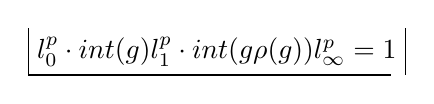
\begin{tikzpicture}[baseline=(m.base)]\node[inner sep=3pt] (m) {$l_0^p\cdot\operatorname{int}(g)l_1^p\cdot\operatorname{int}(g\rho(g))l_\infty^p=1$};\draw (m.north west)--(m.south west)--([xshift=-.18cm]m.south east);\draw (m.north east)--(m.south east);\end{tikzpicture}}
ou encore
\[
l_0^p(gl_1^pg^{-1})(g\rho(g)l_\infty^p\rho(g)^{-1}g^{-1})=1
\]
i.e.
\[
l_0^pgl_1^p\rho(g)l_\infty^p\rho(g)^{-1}g^{-1}=1
\]
soit encore, en faisant passer le $g^{-1}$ à gauche
\[
\deleted{l_0^p\cdot\operatorname{int}(g)\bigl(l_1^p\cdot\operatorname{int}(\rho(g))(l_\infty^p)\bigr)=1}
\]
\[
\operatorname{int}g^{-1})l_0^p\cdot l_1^p\cdot\operatorname{int}(\rho(g)(l_\infty^p)=1
\]
Les relations $\unsure{(*)2|(*)_2|(*),}$ et $(**)$ sont vérifiées par construction (pour $**$, il suffit $\bar m$ de la vérifier pour la valeur aux deux mb en $l_0\ l_1$).
\mspage{7}

\scanpage{9}
\mspage{3}
Mais comment vérifier que $(p;g)$ définissent non seulement un endomorphisme, mais un automorphisme ? Ça semble délicat\ldots

Dans le cas de $\tau$, on a $p=-1$, et $g=l_1$ :
\[
\tau\rho=\operatorname{int}(l_1)\rho\tau
\]
On veut exprimer la commutation de $u$ (comme autom ext \inserted{respectant la structure à lacets}) non seulement à $\rho$ i.e. $\unsure{\mathfrak S_3^+|\mathcal S_3^+}$,
\margin{\uline{NB} Ceci implique qu'il opère \unsure{triv\textsuperscript{t}} sur l'ens. des trois classes de conjugaison des ss-groupes de lacets --- ce qui précède s'applique.}
mais à $\unsure{\mathfrak S_3|\mathcal S_3}$ tout entier. Il suffit d'exprimer la commutation mod autom extérieurs \unsure{à|:} $\sigma_\infty$, i.e. d'écrire qu'il existe $h\in\pi$ (également unique) tel que
\[
u\sigma_\infty=\operatorname{int}(h)\deleted{\unsure{u|\tau}}\sigma_\infty u,
\]
et il suffira de l'exprimer pour les arguments $l_0$ et $l_1$. On trouve les conditions
\[
\underset{\substack{\Vert\\\underbrace{u(l_1)}_{\operatorname{int}(g)l_1^p}}}{u\sigma_\infty(l_0)}=\operatorname{int}(h)\underbrace{\sigma_\infty(l_0^p)}_{l_1^p}
\qquad\text{i.e.}\quad\operatorname{int}(g^{-1}h)l_1^p=l_1^p\quad\text{i.e.}
\]
\[
g^{-1}h\in L_1\quad\text{i.e.}\quad \begin{gathered}[t]h=gl_1^q\\q\in\hat{\mathbb Z}\end{gathered}
\]
et
\[
u\underbrace{\sigma_\infty(l_1)}_{l_0}=\operatorname{int}(h)\sigma_\infty\underbrace{u(l_1)}_{\operatorname{int}(g)l_1^p}\qquad\text{i.e.}
\]
\[
l_0^p=\operatorname{int}(h\sigma_\infty(g))l_0^p\qquad\text{soit}
\]
\[
l_0^p=\operatorname{int}(gl_1^q\sigma_\infty(g))l_0^p\qquad\text{ce qui équivaut à}
\]
\[
\deleted{\operatorname{int}(\unsure{gl_1^q}\sigma_\infty g)L_1=L_0}\qquad\text{i.e. la condition}
\]
\[
\exists_q\ \text{tel que}\quad gl_1^q\sigma_\infty(g)\in L_0
\]
\mspage{8}

\scanpage{10}
ou encore
\[
\exists\ q,r\in\hat{\mathbb Z}^{*}\quad\text{tels que}\quad\boxed{gl_1^q\sigma_\infty(g)=l_0^r}
\]
\margin{il vaut mieux écrire la relation sous la forme
\[
\sigma_\infty(g^{-1})=l_0^\beta gl_1^\gamma,
\]
on trouve, en passant au groupe abélien $\beta=\gamma$ (i.e. $q=-r$) donc
\[
\sigma_\infty(g^{-1})=l_0^\beta gl_1^\beta
\]}
(Condition qui ne dépend que de $g$, pas de $p$;

Si $g$ est remplacé par $g'=l_0^\alpha gl_1^{-\alpha}$, on aura $\sigma_\infty(g')=l_1^\alpha\sigma_\infty(g)l_0^{-\alpha}$, et la relation
\[
g'l_1^{q'}\sigma_\infty(g')=l_0^{r'}
\]
s'écrit
\[
l_0^\alpha gl_1^{-\alpha}l_1^{q'}l_1^\alpha\sigma_\infty(g)l_0^{-\alpha}=l_0^{r'}
\]
i.e. en simplifiant
\[
gl_1^{q'}\sigma_\infty(g)=l_0^{r'}
\]
donc $q=q'$, $r=r'$ i.e. $(q,r)$ ne dépendent que de l'autom ext. défini par $u$, et pas du \deleted{\unsure{choix de u|choix de ce}} de son représentant dans le normalisateur de $L_0$.

Dans le cas de $\tau$, où $g=l_1$, la relation devient
\[
l_1l_1^ql_0\unsure{=|=:}l_0^r\quad\text{donc}\quad q=-1,\ r=1.
\]
On sait que, si on travaille sur les groupes discrets, en plus de l'autom ext. identique, il n'y a qu'une seule autre solution de nos équations (en exigeant \inserted{donc $p=\pm1$ \unsure{et|et)}} que $l_0^p$ et $\operatorname{int}(g)l_1^p$ engendrent $\pi$, en plus des relations fondamentales
\mspage{9}

\scanpage{11}
\mspage{\unsure{4|9}}
plus haut, \deleted{\unsure{pour $g$}} \inserted{savoir $\unsure{\tau|\zeta}$}, \unsure{correspond.|correspond.\textsuperscript{t}} \deleted{\unsure{aux}} à
\[
\left\{\begin{aligned}
p&=-1\qquad g=l_0^\alpha l_1^\beta\quad(\alpha+\beta=1),\ \alpha,\beta\in\mathbb Z)\\
q&=-1,\ r=1\qquad\text{ou mieux, }\beta=-1
\end{aligned}\right.
\]

\uline{NB} Si on remplace dans les calculs qui précèdent $L_0$ par $L_1$, alors $g$ est remplacé par $\rho(g)$, $q$ et $r$ restant inchangés. On trouve ainsi, en plus du caractère cyclotomique $\chi$, \deleted{\unsure{deux}} \inserted{une} \unsure{fonction|fonctions} numérique \inserted{\uline{$\beta$},} sur le groupe
\[
\operatorname{Aut\,ext}_{\mathrm{lac}}(\overset{\pi}{\overset{\Vert}{\hat\pi_{0,3}}},\unsure{\mathfrak S_3|\mathcal S_3})\overset{\unsure{\mathrm{dfn}|\mathrm{def}}}=\Gamma,
\]
\deleted{\unsure{donnée|savoir}} \inserted{à} valeurs dans $\hat{\mathbb Z}$, et une autre \inserted{$\gamma$} \unsure{à|:} valeurs dans $\pi/\hat{\mathbb Z}$, en faisant opérer $\hat{\mathbb Z}$ sur $\pi$ par une opération $\varphi$
\[
\varphi(\alpha)\cdot g=l_0^\alpha gl_1^{-\alpha}
\]
L'application
\[
(\gamma,\chi):\quad\Gamma\longrightarrow\pi/\hat{\mathbb Z}\times\hat{\mathbb Z}^{*}
\]
\[
u\longmapsto(\gamma(u),\chi(u))
\]
\margin{\uline{NB} \inserted{$\gamma_0:\mathcal E_0\longrightarrow\pi$} est un $1$. cocycle sur $\mathcal E_0\unsure{=|\simeq}\operatorname{Aut}_{\mathrm{lac}}(\pi,L_0)$, [\deleted{\unsure{groupe|fixant}} \inserted{qui définit} le ss-gr. des éléments qui commutent ext. à $\unsure{\mathfrak S_3|\mathcal S_3}$}
est injective, \deleted{\unsure{et|$\beta$}} $\beta$ étant défini par $\gamma$ car $\gamma$ prend ses valeurs dans les classes des $g\in\pi$ (mod $\varphi(\hat{\mathbb Z})$) satisfaisant une relation
\mspage{10}

\scanpage{12}
\[
\sigma_\infty(g^{-1})=l_0^\beta g l_1^\beta.
\]
Ce qui détermine $\beta$ de façon unique en fonction de $g$.

\deleted{\unsure{Appliquant|Appliquons} la relation fondamentale}
\[
\deleted{\displaystyle u\unsure{g|\rho}=\operatorname{int}(g)\rho u}
\]
\deleted{à $L_0$, on trouve, puisque $u(L_0)=L_0$, $\rho(L_0)=L_1$}
\[
\deleted{\displaystyle u(L_1)=\operatorname{int}(g)(L_{\unsure{1|0}})}
\]
\deleted{et ceci détermine déjà \deleted{\unsure{$\operatorname{int}(g)$}} \unsure{$g$|\deleted{$g$}} modulo multiplication à droite par un élt de $L_1$, \unsure{par|près|puis} le donnée de $u$}

On a des plus jolis générateurs de \unsure{la|l'} \inserted{sous-}extension de $\unsure{\mathfrak S_3|\mathcal S_3}$ par $\unsure{\pi|\Pi}$ \inserted{dans $\operatorname{Aut}_{\mathrm{lac}}(\unsure{\pi|\Pi})$,} que les six générateurs $l_0,l_1,l_\infty,\sigma_0,\sigma_1,\sigma_\infty$ (donnant $\rho$ par $\sigma_0\sigma_1=l_1^{-1}\rho$ \deleted{\unsure{p.ex.}} i.e. $\rho=\sigma_0\sigma_1l_1$ p.ex), en introduisant les groupes de ramification dans les pts $0,1,\infty$, qui sont canoniq\textsuperscript{t} isomorphes \unsure{à|:} $\widehat{\mathbb Z}$,
On définira donc $\varepsilon_0,\varepsilon_1,\varepsilon_\infty$ par les relations
\[
\varepsilon_0^2=l_0,\qquad\varepsilon_1^2=l_1,\qquad\varepsilon_\infty^2=l_\infty
\]
et plus précisément, $\varepsilon_i$ sera l'unique \deleted{\unsure{él\textsuperscript{t}}} \inserted{autom.} dans la classe mod $\unsure{\pi|\Pi}$ des $\sigma_i$, \deleted{et} qui fixe $l_i$ et est \unsure{\deleted{\unsure{de|$\sigma$}}|$\sigma$} \inserted{\unsure{de carré $l_i$}}
\mspage{11}

\scanpage{13}
Comme $\operatorname{int}(l_0)\sigma_\infty$ fixe\textsuperscript{\unsure{6|$\sigma$}} $l_\infty$ (mais n'est peut-être pas de carré $l_\infty$), on doit le multiplier à droite par un $\operatorname{int}(l_\infty^\alpha)$
\figure{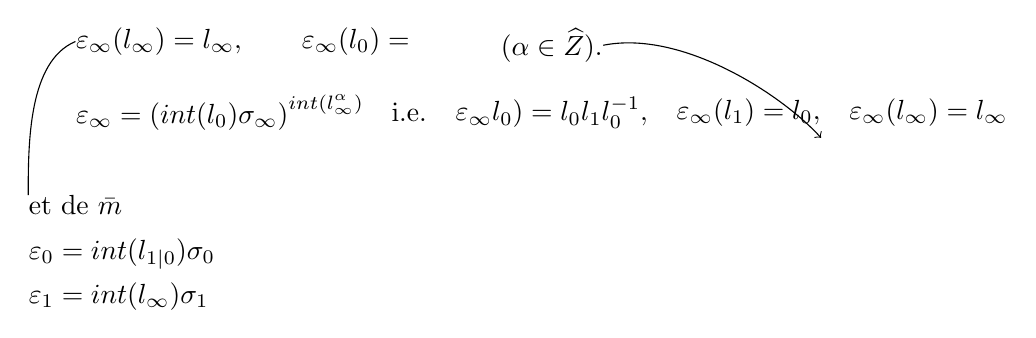
\begin{tikzpicture}[x=1cm,y=1cm]
\node[anchor=west,inner sep=0pt] (def) at (0,0) {$\varepsilon_\infty=(\operatorname{int}(l_0)\sigma_\infty)\raisebox{1.2ex}{$\scriptstyle\inserted{\operatorname{int}(l_\infty^\alpha)}$}$};
\node[anchor=west,xshift=10pt,inner sep=0pt] (ie) at (def.east) {i.e.};
\node[anchor=west,xshift=10pt,inner sep=0pt] (a0) at (ie.east) {$\varepsilon_\infty l_0)=l_0l_1l_0^{-1},$};
\node[anchor=west,xshift=10pt,inner sep=0pt] (a1) at (a0.east) {$\varepsilon_\infty(l_1)=l_0,$};
\node[anchor=west,xshift=10pt,inner sep=0pt] (ai) at (a1.east) {$\varepsilon_\infty(l_\infty)=l_\infty$};
\node[anchor=west,inner sep=0pt] (cancel) at (0,.9) {$\deleted{\varepsilon_\infty(l_\infty)=l_\infty,\qquad\varepsilon_\infty(l_0)=}$};
\node[anchor=south,yshift=12pt,inner sep=0pt] (cond) at (a0.north) {$(\alpha\in\widehat{\mathbb Z})$.};
\draw[->] (cond.east) .. controls +(1.0,.2) and +(-.5,.55) .. ([yshift=-4pt]a1.south east);
\node[anchor=north west,align=left,inner sep=0pt] (other) at (-.6,-1.05) {\deleted{et de $\bar m$}\\[4pt]
$\deleted{\varepsilon_0=\operatorname{int}(l_{\unsure{1|0}})\sigma_0}$\\[4pt]
$\deleted{\varepsilon_1=\operatorname{int}(l_\infty)\sigma_1}$};
\draw (cancel.west) .. controls +(-.6,-.25) and +(0,.65) .. (other.north west);
\end{tikzpicture}}
On \deleted{aura \unsure{donc}} \inserted{doit écrire $\varepsilon_{\unsure{\infty|0}}^2=l_\infty$..} Ecrivant $g$ au lieu de $\operatorname{int}(g)$ pour $g\in\unsure{\pi|\Pi}$, i.e. identifiant $\unsure{\pi|\Pi}$ à un ss-groupe de $\operatorname{Aut}(\unsure{\pi|\Pi})$, je \deleted{\unsure{trouve}} \inserted{\unsure{écris}}
\deleted{\unsure{comme} $\varepsilon_\infty=l_0\sigma_\infty$}.
\[
\varepsilon_\infty=l_0\sigma_\infty l_\infty^\alpha.
\]
\[
\deleted{\displaystyle
\varepsilon_\infty^2=l_0\sigma_\infty l_0\sigma_\infty
=l_0\sigma_\infty l_0\sigma_\infty^{-1}=l_0\sigma_\infty(l_0)
}
\]
donc
\[
\begin{aligned}
\varepsilon_\infty^2&=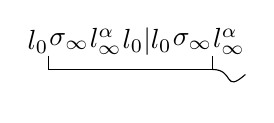
\begin{tikzpicture}[baseline=(a.base)]
\node[inner sep=0pt] (a) at (0,0) {$l_0$};
\node[anchor=west,inner sep=0pt] (b) at (a.east) {$\sigma_\infty$};
\node[anchor=west,inner sep=0pt] (c) at (b.east) {$l_\infty^\alpha$};
\node[anchor=west,inner sep=0pt] (d) at (c.east) {$\unsure{l_0|\deleted{l_0}}$};
\node[anchor=west,inner sep=0pt] (e) at (d.east) {$\sigma_\infty$};
\node[anchor=west,inner sep=0pt] (f) at (e.east) {$l_\infty^\alpha$};
\draw ([yshift=-2pt]b.south west)--([yshift=-7pt]b.south west)--([yshift=-7pt]e.south east)--([yshift=-2pt]e.south east);
\draw ([yshift=-7pt]e.south east) .. controls +(8pt,0) and +(-8pt,-7pt) .. ([yshift=-7pt]f.south east);
\end{tikzpicture}\\
&=l_0\sigma_\infty(l_\infty^\alpha l_0)l_\infty^\alpha
=l_0(l_0^{-1}l_1^{-1})^\alpha l_1(l_1^{-1}l_0^{-1})^\alpha\\
&=\underbrace{\deleted{l_0\sigma_\infty(l_\infty)}}_{\inserted{l_0l_\infty.}}\deleted{\sigma_\infty(l_\infty)^{\alpha-1}\sigma_\infty(l_0)l_\infty^\alpha}
\end{aligned}
\]
et la relation $\varepsilon_\infty^2=l_\infty$ \inserted{\deleted{$\unsure{(=)|(\Rightarrow)}l_1^{-1}l_{\unsure{0|\infty}}^{-1}$}} s'écrit aussi, en multipliant par $l_0l_1$
\[
\deleted{\displaystyle
l_0l_\infty\underbrace{\sigma_\infty(l_\infty)^{\alpha-1}}_{(l_0^{-1}l_1^{-1})^{\alpha-1}}\underbrace{\sigma_\infty(l_0)}_{l_1}l_\infty^{\alpha-1}=1
}
\]
i.e.
\[
\deleted{\displaystyle
\deleted{\unsure{l_\infty^{-1}l_1|l_\infty^{-1}l_\infty|l_0^{-1}l_1}}l_0^{1-\alpha}l_1^{2-\alpha}l_\infty^\alpha=1
}
\]
\[
l_0l_1l_0(l_0^{-1}l_1^{-1})^\alpha l_1(l_1^{-1}l_{\unsure{0|\infty}}^{-1})^\alpha=1
\]
\margin{\unsure{prends|prenons|pour} $\alpha\unsure{=|\ge}\unsure{2|1}$ ?}
\[
\deleted{\displaystyle
l_0l_1l_0l_0^{-1}l_1^{-1}l_0^{-1}l_1^{-1}l_1l_1^{-1}l_0^{-1}l_1^{-1}l_0^{-1}=1?\qquad\text{Non !}
}
\]
\[
\deleted{l_0}\deleted{l_1}\deleted{l_0}\deleted{l_0^{-1}}\deleted{l_1^{-1}}\deleted{l_1}\deleted{l_1^{-1}}\deleted{l_0^{-1}}=1
\qquad\text{OK}\qquad\text{donc}
\]
\[
\left\{\begin{aligned}
\varepsilon_\infty&=l_0\sigma_\infty l_\infty\quad\text{(ou encore }\operatorname{int}(l_0)\sigma_\infty\operatorname{int}(l_\infty)\text{)}\\
\varepsilon_0&=l_1\sigma_0l_0\\
\varepsilon_1&=l_\infty\sigma_1l_1
\end{aligned}\right.
\]
\mspage{12}

\scanpage{14}
donc
\[
\begin{aligned}
\varepsilon_0^2&=l_0\\
\varepsilon_1^2&=l_1\\
\varepsilon_\infty^2&=l_\infty
\end{aligned}
\]
Ce qui redonne les $l_i$, et aussi les $\sigma_i$, \deleted{\unsure{par}} en termes des $\varepsilon_i$
\[
\begin{aligned}
\sigma_0&=\varepsilon_0\varepsilon_1^2\\
\sigma_1&=\varepsilon_1\varepsilon_\infty^2\\
\sigma_\infty&=\varepsilon_\infty\varepsilon_0^2
\end{aligned}
\]
D'où les relations
\[
\left\{\begin{aligned}
\varepsilon_0^2\varepsilon_1^2\varepsilon_\infty^2&=1\\
(\varepsilon_0\varepsilon_1^2)^2&=1\\
(\varepsilon_1\varepsilon_\infty^2)^2&=1\\
(\varepsilon_\infty\varepsilon_0^2)^2&=1
\end{aligned}\right.
\]
On retrouve $\rho$ \deleted{\unsure{comme}} par
\[
\begin{array}{r@{}c@{}l}
\deleted{\rho={}}&\deleted{\sigma_0\sigma_1}&\deleted{{}=\sigma_1\sigma_\infty=\sigma_\infty\sigma_0}\\
&\Vert&\\
&\makebox[0pt][c]{$\deleted{\varepsilon_0\varepsilon_1^3\unsure{\varepsilon_\infty|\varepsilon_0|\varepsilon_1}}$}&
\end{array}
\]
\[
\inserted{\sigma_0\sigma_1=l_1^{-1}\rho}
\]
\margin{donc
\[
\begin{aligned}
\rho&=l_1\sigma_0\sigma_1\\
&=\varepsilon_1^2\varepsilon_0\varepsilon_1^2\varepsilon_1\varepsilon_\infty^2\\
&=\varepsilon_1^2\varepsilon_0\varepsilon_1^{\deleted{\unsure{2|3}}}\underbrace{\varepsilon_1^2\varepsilon_\infty^2}_{\varepsilon_0^{-2}}
\end{aligned}
\]}
\[
\begin{aligned}
\rho&=\varepsilon_1^2\varepsilon_0\varepsilon_1\varepsilon_0^{-2}\\
&=\varepsilon_\infty^2\varepsilon_1\varepsilon_\infty\varepsilon_1^{-2}\\
&=\varepsilon_0^2\varepsilon_\infty\varepsilon_0\varepsilon_\infty^{-2}:
\end{aligned}
\]
\margin{\begin{tabular}{|l}
ces relations ne\\
semblent pas conséquences\\
des autres
\end{tabular}}
multipliant \deleted{\unsure{dans|donc}} ces relations dans l'ordre inverse et écrivant $\rho^3=1$, on trouve
\[
(\varepsilon_0\varepsilon_1\varepsilon_\infty)^2=1
\]
ce qui est inquiétant, car il n'y a pas d'\unsure{élém\textsuperscript{ts}}
\mspage{13}

\scanpage{15}
\deleted{d'ordre fini dans le groupe envisagé \inserted{\deleted{\unsure{stable|stables}} fixé par $\rho$}, il faudrait donc avoir}
\[
\deleted{\displaystyle \varepsilon_0\varepsilon_1\varepsilon_\infty=1}
\]
\deleted{i.e. en termes des $l_i,\sigma_i$}
\[
\deleted{\displaystyle \unsure{l_1|l_1'}\underbrace{\sigma_0l_0}_{\substack{\inserted{\deleted{l_{\unsure{1}}\sigma_\infty}}\\\deleted{l_1^{-1}l_\infty^{-1}\sigma_0}}}l_\infty\underbrace{\sigma_1l_1}_{l_\infty^{-1}l_0^{-1}}l_0\underbrace{\sigma_\infty l_\infty}_{l_0^{-1}l_1^{-1}}=1}
\]
\margin{\deleted{i.e. $l_\infty^{-1}l_0^{-1}l_1^{-1}=1$\quad OK}}
\deleted{On a donc}
\[
\deleted{\displaystyle \boxed{\varepsilon_0\varepsilon_1\varepsilon_\infty=1}}
\]
\deleted{on peut en tirer de plus jolies expressions pour les $\sigma_i$}
\[
\begin{aligned}
\deleted{\displaystyle \sigma_0}&\deleted{\displaystyle =\varepsilon_\infty^{-1}\varepsilon_1}\\
\deleted{\displaystyle \sigma_1}&\deleted{\displaystyle =\varepsilon_0^{-1}\varepsilon_\infty}\\
\deleted{\displaystyle \sigma_\infty}&\deleted{\displaystyle =\varepsilon_1^{-1}\varepsilon_0}
\end{aligned}
\]
\deleted{donc \unsure{aussi|on a} la relation inattendue}
\[
\deleted{\displaystyle \sigma_\infty\sigma_1\sigma_0=1}
\]
Sans doute
\[
\varepsilon_0\varepsilon_1\varepsilon_\infty=\sigma_1
\]
i.e.
\[
\begin{aligned}
\varepsilon_0&=\varepsilon_1\varepsilon_\infty\varepsilon_{\unsure{1}}^{-1}\\
\varepsilon_1&=\varepsilon_\infty\varepsilon_0\varepsilon_\infty^{-1}\\
\varepsilon_\infty&=\varepsilon_0\varepsilon_1\varepsilon_0^{-1}
\end{aligned}
\]
\figure{\begin{tikzpicture}\draw (0,0)--(.15,0);\draw (.25,0)--(.8,0);\end{tikzpicture}}

Critique des notations et de l'approche. Les éléments $l_i,\sigma_i,\varepsilon_i,\rho\ldots$ sont dans les groupes discrets, qu'il faudrait distinguer des groupes profini --- de plus il faudrait pour les groupes discret \deleted{\unsure{utiliser}} \unsure{(et|Cat} $\bar m$ pour les
\mspage{14}

\scanpage{16}
profinis, dans une certaine mesure !) utiliser le langage géométrique des groupoïdes fondamentaux de $\mathbb P^1(\mathbb C)-\{0,1,\infty\}$. On \deleted{\unsure{pourra|posera}} notera donc $\Pi=\Pi_{0,3}$ le groupe discret
\[
\Pi=\Pi_{\unsure{1|*}}(\overbrace{\mathbb P^1(\mathbb C)\setminus\{0,1,\infty\}}^{U=U_{0,3}},P)
\]
où $\mathbb P^1(\mathbb C)$ est muni de la structure \inserted{de sphère} riemannienne \inserted{orientée} unique pour laquelle la rotation \inserted{$\dot\rho$} d'angle $+\frac{2\pi}{3}$ autour de l'axe $P,\bar P$ \deleted{\unsure{qui}} induit sur $(0,1,\infty)$ la permutation circulaire $0\longrightarrow1\longrightarrow\infty\longrightarrow0$ Ceci correspond à l'orientation habituelle de la sphère), et où les aut complexes \inserted{$\dot\sigma_0,\dot\sigma_1,\dot\sigma_\infty$} de $\mathbb P^1_{\mathbb C}$ qui \deleted{\unsure{échangent}} \inserted{\deleted{\unsure{fixent}}} \unsure{induisent|deux $p^t$} \deleted{\unsure{resp|sur}.} sur $(0,1,\infty)$ les transpositions fixant resp. $0,1,\infty$, sont \inserted{resp.} les \deleted{\unsure{rotations}} \inserted{symétries} autour des axes \deleted{$\unsure{P,\bar P|1,\infty|0,1,\infty}$} $(0,2)$, $(1,-1)$ et $(\infty,\frac12)$.
\margin{Sur la sphère de Riemann on a
\[
\begin{aligned}
\sigma_0(z)&=\frac{-\unsure{z|1}}{1-z}=\frac{z}{z-1}\\
\sigma_1(z)&=\frac1z\\
\sigma_\infty(z)&=1-z\\
\rho(z)&=\frac1{1-z}\\
\rho^2(z)&=1-\frac1z
\end{aligned}
\]}
Quant à la conjugaison complexe, c'est la symétrie p.r. \unsure{au|un} plan $(0,1,\infty)$. On considère $\unsure{\mathfrak S_3|\mathcal S_3}$ comme opérant sur $(0,1,\infty)$ \unsure{dans|ds} cet ordre, et $\unsure{\mathfrak S_3|\mathcal S_3}\times\mathbb Z/2$ comme opérant sur la sphère; via les $\dot\sigma_0,\dot\sigma_1,\dot\sigma_\infty\in\unsure{\mathfrak S_3|\mathcal S_3}$ et $\dot\tau\in\mathbb Z/2$. On considère l'extension \inserted{$\deleted{\unsure{\mathcal E_0}}$} de $\unsure{\mathfrak S_3|\mathcal S_3}\times\mathbb Z/2$ par $\Pi$, notée \inserted{$\mathcal E_{0,3}$ ou} $\mathcal E$, définie par
\[
\mathcal E=\Pi_1\left(\underset{\substack{\Vert\\U_{0,3}}}{U_{\deleted{\unsure{0,3}}}},\underbrace{\unsure{\mathfrak S_3|\mathcal S_3}\times\mathbb Z/2}_{\Gamma};P\right)
\]
\mspage{15}

\scanpage{17}
\mspage{7}
Le groupe fondamental mixte est défini à la Malgoire, \deleted{\unsure{correspondant|comprenant}} les classes $(\gamma,\unsure{l|\lambda})$ d'un $\gamma\in\Gamma$ et d'une classe de chemins $l$\unsure{/|)}de $P$ dans $\gamma^{-1}(P)$, en définissant
\[
(\gamma,l)(\gamma',l')=(\inserted{\gamma\gamma',}\gamma'^{-1}(l)\circ l')
\]
i.e. ``composant les chemins comme des fonctions'' (c'est la convention pour faire opérer \uline{\unsure{à|:} gauche} le groupoïde fondamental sur les fibres d'un rev. étale \inserted{$U'$}, à une classe de chemins $l$ de $x$ à $y$ étant associé $l_\bullet:U'_{\unsure{a|x}}\longrightarrow U'_y\ldots$)

On choisit des éléments
\[
\sigma_0,\sigma_1,\sigma_\infty\qquad\text{sur}\qquad\dot\sigma_0,\dot\sigma_1,\dot\sigma_\infty
\]
comme les couples d'un $\sigma_i$, et des chemins \inserted{$\lambda_i$} de $P$ \unsure{à|:} $\bar P=\sigma_iP$ qui se fait sur \deleted{l'unique} \inserted{celui des} demi-grands cercles de $P$ à $\bar P$, \deleted{stable par \unsure{à|$\dot\tau$} la symétrie} \inserted{ens. des pts fixes} \deleted{$\tau\sigma_i$} de la symétrie $\dot\tau\dot\sigma_i=\dot\sigma_i\dot\tau$ (symétrie p.r. \unsure{au|à un|à} plan, fixant $P,\bar P,a_i$ $(=0,1\text{ ou }\infty)$ et échangeant les deux autres $a_j,a_k$) et \unsure{ne|un|en} passant pas par $a_i$. \deleted{\unsure{Au}} Désignant par $l_0,l_1,l_\infty$ \inserted{(pour $1\in\Gamma$)} les lacets en sens direct autour des $0,1,\infty$ à partir de $P$, en allant vers $\unsure{a_0,a_1,a_\infty|0,1,\infty}$ suivant des des quarts de grands cercles, on trouve
\[
(1)\qquad\big|\quad l_\infty\unsure{l'_1|l_1}l_0=1
\]
(et non $l_0l_1l_\infty=1$ ! \unsure{\}|?|)} On peut l'écrire $l_0^{-1}l_1^{-1}l_\infty^{-1}=1$)
et les relations
\mspage{16}

\scanpage{18}
\[
(2)\quad\left\{\begin{gathered}
\sigma_0^2=\sigma_1^2=\sigma_\infty^2=1\\
\sigma_0\sigma_1=\deleted{\unsure{l_0\rho}}\inserted{\rho l_0}\qquad
\unsure{\sigma_1|\dot\sigma_1}\sigma_\infty=\deleted{\unsure{l_1\rho}}\inserted{\rho l_1}\qquad
\sigma_\infty\sigma_0=\deleted{l_\infty\rho}\inserted{\rho l_\infty}
\end{gathered}\right.
\]
\margin{NB Comme $\sigma_1=\rho\sigma_0\rho^{-1}\ldots$, ces $\leftarrow$ relations s'écrivent aussi
\[
\begin{aligned}
\deleted{\displaystyle l_0}&\deleted{\displaystyle =(\sigma_0\rho)^2\unsure{\sigma_\infty}(\unsure{l_0\sigma_0\sigma_0\rho^{-1}|\rho\sigma_0\rho^{-1}})}\\
\deleted{\displaystyle l_1}&\deleted{\displaystyle =(\sigma_1\rho)^2\unsure{\sigma_1}\qquad}&\deleted{\displaystyle \unsure{l_0}}&\deleted{\displaystyle =\unsure{\rho^{-1}\sigma_0}}\\
\deleted{\displaystyle l_\infty}&\deleted{\displaystyle =(\sigma_\infty\rho)^2\unsure{\sigma_\infty}}
\end{aligned}
\]
\begin{tabular}{|l}
$\begin{aligned}
l_0&=\rho^{-1}\sigma_0\rho\sigma_0\rho^{-1}\\
\text{\deleted{On a}}&=\rho^{-1}[\sigma_0,\rho]
\end{aligned}$\\
On a\\
$\begin{aligned}
\deleted{\sigma_0(l_0)=l_1}\\
\deleted{\sigma_0(l_1)=\unsure{l_\infty|l_0}}\\
\deleted{\sigma_0(l_\infty)=\unsure{l_1^{-1}l_0^{-1}}}
\end{aligned}$\\
$\begin{aligned}
\sigma_0(l_0)&=l_\infty^{-1}l_1^{-1}\\
\sigma_0(l_1)&=l_\infty
\end{aligned}$
\end{tabular}
\[
\sigma_0(l_\infty)=l_1
\]}
où $\rho$, au dessus de $\dot\rho$, est défini par le chemin trivial de $P$ \unsure{à|:} $P$. On a donc
\[
\left\{\begin{aligned}
\rho\sigma_0\rho^{-1}&=\sigma_1\\
\rho\sigma_1\rho^{-1}&=\sigma_\infty\\
\rho\sigma_\infty\rho^{-1}&=\sigma_0
\end{aligned}\right.
\qquad\text{i.e}\quad
\left\{\begin{aligned}
\rho\sigma_0&=\sigma_1\rho\\
\rho\sigma_1&=\sigma_\infty\rho\\
\rho\sigma_\infty&=\sigma_0\rho
\end{aligned}\right.
\]
On ne voit pas apparaître d'expression de $\rho$ en fonction des $\sigma_0,\sigma_1,\sigma_\infty$ seuls --- \deleted{on voit par contre (utilisant le fait que $l_0,l_1,l_\infty$ avec \mbox{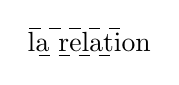
\begin{tikzpicture}[baseline=(relation.base)]
\node[inner sep=0pt,outer sep=0pt] (relation) {la relation};
\draw ([xshift=0.05em,yshift=0.35ex]relation.north west) -- ++(0.42em,0);
\draw ([xshift=0.77em,yshift=0.35ex]relation.north west) -- ++(0.42em,0);
\draw ([xshift=1.49em,yshift=0.35ex]relation.north west) -- ++(0.42em,0);
\draw ([xshift=2.21em,yshift=0.35ex]relation.north west) -- ++(0.42em,0);
\draw ([xshift=2.93em,yshift=0.35ex]relation.north west) -- ++(0.42em,0);
\draw ([xshift=0.40em,yshift=-0.35ex]relation.south west) -- ++(0.42em,0);
\draw ([xshift=1.12em,yshift=-0.35ex]relation.south west) -- ++(0.42em,0);
\draw ([xshift=1.84em,yshift=-0.35ex]relation.south west) -- ++(0.42em,0);
\draw ([xshift=2.56em,yshift=-0.35ex]relation.south west) -- ++(0.42em,0);
\end{tikzpicture}} fondamentale (1) est une présentation de $\unsure{\Pi|\pi}$, que \deleted{$\rho$} \inserted{$(\sigma_0\sigma_1)^3$ (p.ex)} doit s'exprimer en fonction des $l_i$; \unsure{puisque} en outre}
\[
\deleted{\displaystyle\deleted{\rho=l_0l_1l_\infty}}
\]
\deleted{des \unsure{relations|rel.} $\sigma_i^2=1$}, il faudra que $\rho$ soit produit de termes $\sigma_i$ \uline{pas deux consécutifs} \deleted{\unsure{distincts|abstrait\textsuperscript{t}}}, \deleted{\unsure{ou|or} $\sigma_0\sigma_1\sigma_0=$} \inserted{et $\sigma$}
\[
\left\{\begin{aligned}
\dot\sigma_1^2=\dot\sigma_{\unsure{1|0}}^2=\dot\sigma_\infty^2&=1\\
\dot\sigma_0\dot\sigma_1=\dot\sigma_1\dot\sigma_\infty=\dot\sigma_\infty\dot\sigma_0&=\dot\rho\\
\dot\rho^3&=1
\end{aligned}\right.
\quad\text{est une présentation de }\unsure{\mathfrak S_3|\mathcal S_3}\text{\unsure{),|,}}
\]
\margin{\begin{tabular}{l}
\unsure{Comme on voit}\\
\unsure{ils|être} \unsure{en|un} \unsure{sont|des}\\
\unsure{\uline{pas} conjugu\uline{és}|\uline{pas} conjugués|\uline{pas} exig\uline{ée}}
\end{tabular}}
que le système des relations (1)(2) et \unsure{outre|enfin|entre}
\[
\rho^3=1
\]
est une présentation de l'image inverse de $\unsure{\mathfrak S_3|\mathcal S_3}$ dans $\mathcal E$ (dis dans $\widehat{\mathcal E}$, au pt de vue profini).
\margin{C'est faux, Comme on voit en faisant dans ces relations $\rho=1$, on \unsure{a} \unsure{pas|plus|puis} $\unsure{\rho\sigma_0\rho^{-1}=\sigma_1}$ (?)}
\mspage{17}

\scanpage{19}
\[
(8)\quad\left\{\begin{aligned}
\varepsilon_0&=l_0^{\deleted{\unsure{-1}}}\sigma_0l_{\unsure{1|0}}^{\deleted{\unsure{-1}}}\\
\varepsilon_1&=l_{\unsure{1|\infty}}^{\deleted{\unsure{-1}}}\sigma_{\unsure{1|\infty}}l_{\unsure{\infty|0}}^{\deleted{\unsure{-1}}}\\
\varepsilon_\infty&=l_\infty\sigma_\infty l_{\unsure{0|\infty}}^{\deleted{\unsure{-1}}}
\end{aligned}\right.
\]
\margin{\uline{NB}\quad $\rho\varepsilon_i\rho^{-1}=\varepsilon_{\dot\rho i}$ i.e
\[
\left\{\begin{aligned}
\rho\varepsilon_0\rho^{-1}&=\varepsilon_1\\
\rho\varepsilon_1\rho^{-1}&=\varepsilon_\infty\\
\rho\varepsilon_\infty\rho^{-1}&=\varepsilon_0
\end{aligned}\right.
\]}
On a bien
\[
\varepsilon_0^2=l_0\underbrace{\sigma_0l_1l_0\sigma_0}_{\substack{\sigma_0(l_1l_0)=\sigma_0(l_1)\sigma_0(l_0)\\=l_\infty(l_1l_\infty)^{-1}=l_1^{-1}}}l_{\unsure{1|0}}=l_0l_\infty l_\infty^{-1}l_1^{-1}l_1=l_0\qquad\text{ok}
\]
(\uline{NB} Les $\varepsilon_i$ ici sont les $\varepsilon_i^{-1}$ de tantôt ! \deleted{\unsure{il faudrait|il faut donc les}} \inserted{qu'il faudra} \deleted{\unsure{ici|laisser}} donc noter $\varepsilon'_i\ldots$)

Ici on voit donc qu'on a un syst. de gén. et relations \inserted{de $\mathcal E^+$} $l_0,l_1,l_\infty,\varepsilon_0,\varepsilon_1,\varepsilon_\infty,\rho$ \deleted{de $\mathcal E^+$}, les relations
\[
\left\{\begin{gathered}
l_\infty l_1l_0=1\\
\varepsilon_0^2=l_0,\quad\varepsilon_1^2=l_1,\quad\varepsilon_\infty^2=l_\infty\\
\varepsilon_0\varepsilon_1=\rho\deleted{\unsure{l_\infty}}(\unsure{..|\ldots}),\quad\varepsilon_1\varepsilon_\infty=\mathinner{..},\quad\varepsilon_\infty\varepsilon_0=\mathinner{.\!-},\quad\rho^3=1
\end{gathered}\right.
\]
où il faut compléter l'expression de $\varepsilon_0\varepsilon_1$ etc \inserted{comme} \unsure{produits|produit|quotient} de $\rho$ par des expressions
\[
\deleted{\displaystyle
\varepsilon_0\varepsilon_1=l_0\sigma_1l_1
}
\]
en les $l_i$.
\[
\varepsilon_0\varepsilon_1=l_0\sigma_0l_1l_1\sigma_1l_\infty
=l_0\underset{l_\infty^2}{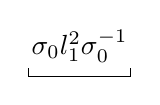
\begin{tikzpicture}[baseline=(term.base)]\node[inner sep=1pt] (term) {$\sigma_0l_1^2\sigma_0^{-1}$};\draw ([yshift=-1pt]term.south west) -- ++(0,-3pt) -| ([yshift=-1pt]term.south east);\end{tikzpicture}}\underset{\rho l_0}{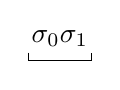
\begin{tikzpicture}[baseline=(term.base)]\node[inner sep=1pt] (term) {$\sigma_0\sigma_1$};\draw ([yshift=-1pt]term.south west) -- ++(0,-3pt) -| ([yshift=-1pt]term.south east);\end{tikzpicture}}l_\infty
=l_0l_\infty^2\rho l_0l_\infty
\]
donc finalement
\[
(9)\quad\left\{\begin{aligned}
\varepsilon_0\varepsilon_1\deleted{\unsure{\varepsilon}}&=l_0l_\infty^2\rho l_0l_\infty\\
\varepsilon_1\varepsilon_\infty&=l_1l_0^2\rho l_1l_0\\
\varepsilon_\infty\varepsilon_0&=l_\infty l_1^2\rho l_\infty l_1
\end{aligned}\right.
\]
Éliminant les $l_i$ comme $\varepsilon_i^2$, on trouve des gén $\varepsilon_0,\varepsilon_1,\varepsilon_\infty,\rho$, avec relations de \unsure{définition|définit}
\mspage{18}

\scanpage{20}
\mspage{8}
Il revient au $=$ de dire que $\sigma_0,\sigma_1,\sigma_\infty,\rho$ sont des générateurs, avec relations de définition
\[
(4)\qquad
(\overbrace{\rho^{-1}\sigma_\infty\sigma_0\deleted{\rho}}^{l_\infty})
(\overbrace{\rho^{-1}\sigma_1\sigma_\infty\deleted{\rho}}^{l_1})
(\overbrace{\rho^{-1}\sigma_0\sigma_1\deleted{\rho}}^{l_0})=1
\]
\[
(5)\qquad \sigma_0^2=\sigma_1^2=\sigma_\infty^2=1
\]
\[
(6)\qquad \rho^3=1
\]
\margin{Il faut ajouter les relations $\rho\sigma_0\rho^{-1}=\sigma_1$ etc
On a deux gén. $\sigma_0,\rho$ en fait avec relations
\[
\sigma_0^2=\rho^3=1,
\]
la
\deleted{$\unsure{[\underset{\sigma_\infty}{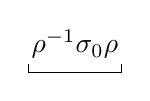
\begin{tikzpicture}[baseline=(term.base)]\node[inner sep=1pt] (term) {$\rho^{-1}\sigma_0\rho$};\draw ([yshift=-1pt]term.south west) -- ++(0,-3pt) -| ([yshift=-1pt]term.south east);\end{tikzpicture}}\sigma_0\rho^{-1}][\underset{\sigma_1}{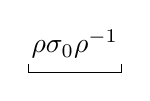
\begin{tikzpicture}[baseline=(term.base)]\node[inner sep=1pt] (term) {$\rho\sigma_0\rho^{-1}$};\draw ([yshift=-1pt]term.south west) -- ++(0,-3pt) -| ([yshift=-1pt]term.south east);\end{tikzpicture}}\underset{\sigma_\infty}{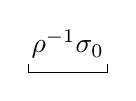
\begin{tikzpicture}[baseline=(term.base)]\node[inner sep=1pt] (term) {$\rho^{-1}\sigma_0$};\draw ([yshift=-1pt]term.south west) -- ++(0,-3pt) -| ([yshift=-1pt]term.south east);\end{tikzpicture}}\rho^{-1}]|[\underset{\sigma_\infty}{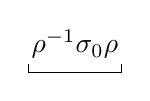
\begin{tikzpicture}[baseline=(term.base)]\node[inner sep=1pt] (term) {$\rho^{-1}\sigma_0\rho$};\draw ([yshift=-1pt]term.south west) -- ++(0,-3pt) -| ([yshift=-1pt]term.south east);\end{tikzpicture}}\sigma_0\rho^{-1}][\underset{\sigma_1}{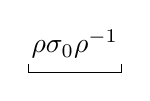
\begin{tikzpicture}[baseline=(term.base)]\node[inner sep=1pt] (term) {$\rho\sigma_0\rho^{-1}$};\draw ([yshift=-1pt]term.south west) -- ++(0,-3pt) -| ([yshift=-1pt]term.south east);\end{tikzpicture}}\underset{\sigma_\infty}{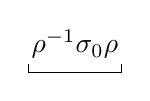
\begin{tikzpicture}[baseline=(term.base)]\node[inner sep=1pt] (term) {$\rho^{-1}\sigma_0\rho$};\draw ([yshift=-1pt]term.south west) -- ++(0,-3pt) -| ([yshift=-1pt]term.south east);\end{tikzpicture}}\rho^{-1}]}$}
relation (4) est conséquence des précédentes (vient du fait $\sigma_1=\rho\sigma_0\rho^{-1}$, \deleted{\illegible{1}} $\sigma_\infty=\rho^{-1}\sigma_0\rho$). Noter que
\[
\begin{aligned}
l_0&=\deleted{\unsure{(\rho\sigma_0\rho^{-1})^2|(\sigma_0\rho)^2}}\rho^{-1}(\sigma_0\rho)^2\rho
=\boxed{\rho^{-1}\sigma_0\rho\sigma_0\rho^{-1}}\\
l_1&=(\deleted{\unsure{\rho}}\sigma_0\rho)^2\\
l_\infty&=(\unsure{\rho^{\deleted{-1}}|\rho^{-1}}\sigma_0\deleted{\unsure{\rho}})^2
\end{aligned}
\]
\[
\begin{aligned}
\operatorname{int}(\sigma_0)l_1&=l_\infty\\
\operatorname{int}(\sigma_0)l_\infty&=l_1\\
\operatorname{int}(\sigma_0)(l_0)&=l_\infty^{-1}l_1^{-1}
\end{aligned}
\]}
\margin{\uline{NB}
\[
\begin{aligned}
\sigma_0(l_0)&=l_\infty^{-1}l_1^{-1}\\
\sigma_0(l_1)&=l_\infty\\
\sigma_0(l_\infty)&=l_1^{\deleted{\unsure{-1}}}\deleted{\unsure{l_\infty^{-1}|l_0^{-1}}}
\end{aligned}
\]
et itou pour $\sigma_1,\sigma_\infty$}
\uline{NB} Si on y fait \inserted{de plus} $\sigma_0,\sigma_1,\sigma_\infty=1$, on trouve comme relation de définition $\rho^3=1$, \deleted{\unsure{donc}} sans plus, ce qui prouve que $\rho$ n'est pas un mot \unsure{p.v.|p.r.} aux $\sigma_i$\ldots

Tout ceci est compatible avec les relations des débuts, \deleted{\unsure{si dans ces dernières on avait tout pris des primes}, et \unsure{qu'on interprète} $l_i'=l_i^{-1}$, $\sigma_i'=\sigma_{\unsure{\dot\rho(i)}}$}
\deleted{i.e. $\sigma_i$} \deleted{\unsure{de notre groupe|de sorte que} $\unsure{\mathcal E'|\sigma_i'|\sigma'}$} si on y remplace les $l_i$ par les $l_i^{-1}$
Ici on a, comme $\sigma_i=\sigma^{\unsure{\prime|1}}_{\dot\rho^{-1}(i)}$
\[
(7)\quad\left\{\begin{aligned}
\operatorname{int}(\sigma_i)&:\text{ échange }l_j\text{ et }l_{\deleted{\unsure{j}}k}
\quad\inserted{(i,j,\unsure{k|h})\text{ distincts})}\ \deleted{\text{et}}\\[-2pt]
&\deleted{\text{(et le }\unsure{\text{dernier}|\text{devenir}}\ l_{\dot\rho(i)}\ \text{s'en déduit par (1))}}\\
\operatorname{int}(\rho)l_i&=l_{\dot\rho(i)}
\end{aligned}\right.
\]

On voudrait maintenant expliciter les $\varepsilon_i$ avec $\varepsilon_i^2=l_i$ $(i=0,1,\infty)$, $\varepsilon_i$ étant \unsure{donc un|un des} \unsure{générateurs|générateur} \unsure{du|des} centralisateur (ou normalisateur, c'est idem) des $L_i$ dans $\mathcal E^+$\unsure{.|,} (ou le centralisateur dans $\mathcal E$). Les calculs faits plus haut, avec les chgts de \unsure{notation|notations} indiqués, donnent
\[
\deleted{(8)}\quad\left\{\begin{aligned}
\unsure{\deleted{\varepsilon_0}|\varepsilon_0}&=l_0^{\deleted{\unsure{-1|4}}}\sigma_1 l_{\unsure{0|1}}^{\deleted{\unsure{-1|4}}}\\
\unsure{\deleted{\varepsilon_1}|\varepsilon_1}&=\unsure{\deleted{l_\infty^{-1}}|l_\infty^{-1}}\sigma_\infty \deleted{l_1^{-1}}\ \inserted{l_1}\\
\varepsilon_\infty&=l_0^{-1}\sigma_0 l_\infty
\end{aligned}\right.
\]
\mspage{19}

\scanpage{21}
Donc on a les relations
\[
(13)\quad\left\{\begin{gathered}
\tilde\sigma_0^2=\tilde\sigma_1^2=\tilde\sigma_\infty^2=1\\
\tilde\sigma_0\tilde\sigma_1=\tilde\sigma_1\tilde\sigma_\infty=\tilde\sigma_\infty\tilde\sigma_0
=\overset{\deleted{\sim}}{\rho}\ \deleted{(\unsure{=\rho})}\\
(\overset{\deleted{\sim}}{\rho}{}^3=1\text{ est conséquence des précédentes})
\end{gathered}\right.
\]
\margin{NB
\[
\rho\tilde\sigma_i\rho^{-1}=\tilde\sigma_{\dot\rho i}\quad\text{i.e}
\]
\[
\begin{aligned}
\rho\tilde\sigma_0\rho^{-1}&=\tilde\sigma_1\\
\rho\tilde\sigma_1\rho^{-1}&=\tilde\sigma_\infty\\
\rho\tilde\sigma_\infty\rho^{-1}&=\tilde\sigma_0
\end{aligned}
\]}
et l'image réciproque $\tilde{\mathcal E}$ de $\varphi(\overset{\deleted{\unsure{\sim}}}{\unsure{\mathfrak S_3|\mathcal S_3}})\subset\Gamma$ (ss-groupe d'indice 2) est produit $\frac12$ direct de $\unsure{\mathfrak S_3|\tilde{\mathfrak S}_3|\mathcal S_3|\tilde{\mathcal S}_3}$ et de $\Pi$. Il faut expliciter les opérations des $\tilde\sigma_a$ sur\unsure{.} $\unsure{\pi|\Pi}$ pour avoir la structure complète du groupe, On trouve que $\tilde\sigma_a$ est au dessus $\varphi(\overset{\deleted{\sim}}{\dot\sigma}_a)$ i.e. la symétrie p.r. au plan passant par $P,\bar P,\deleted{\unsure{a_i|\infty|a}}i$, qui transforme $l_0$ en $l_0^{-1}$, $\deleted{l}l_\infty$ en $l_{\unsure{1|0}}^{-1}$, $l_1$ en $l_\infty^{-1}$ :
\margin{Ce sont celles obtenues par transport de structure, via les opérations de $\unsure{\mathfrak S_3|\tilde{\mathfrak S}_3|\mathcal S_3|\tilde{\mathcal S}_3}$ sur $(U,P)$}
\[
(14)\quad\left\{\begin{array}{lll}
\tilde\sigma_0l_0\tilde\sigma_0^{-1}=l_0^{-1}&
\tilde\sigma_0l_1\tilde\sigma_0^{-1}=l_\infty^{-1}&
\tilde\sigma_0l_\infty\tilde\sigma_0^{-1}=l_1^{-1}\\
\tilde\sigma_1l_1\tilde\sigma_1^{-1}=l_1^{-1}&\begin{tikzpicture}[baseline=-0.4ex,x=1em,y=1ex]
\fill (0,0.12)--(0.08,0.32)--(0.15,0.11)--(0.31,0.06)--(0.16,-0.05)--(0.13,-0.22)--(0.04,-0.08)--(-0.09,-0.06)--cycle;
\draw[line width=0.55pt] (0.50,0)--(0.70,0) (0.98,0)--(1.18,0) (1.46,0)--(1.66,0);
\end{tikzpicture}&\\
\begin{tikzpicture}[baseline=-0.4ex,x=1em,y=1ex]
\draw[line width=0.55pt] (0,0)--(0.20,0) (0.48,0)--(0.68,0) (0.96,0)--(1.16,0) (1.44,0)--(1.64,0);
\end{tikzpicture}&&
\end{array}\right.
\]
\margin{\uline{Critique} La n. $\tilde\sigma_0$ suggère plutôt que $\tilde\sigma_0$ est au dessus de $\sigma_0$ --- il vaut mieux écrire $\dot\sigma_i'=\dot\sigma_i\tau$ et noter $\tilde\sigma_i'$ au lieu de $\tilde\sigma_i$ $(i\in\{0,1,\infty\})$, ou mieux $\sigma_i'$ (sans $\sim$) --- pour réserver $\tilde\sigma_i'$ à des éléments de $S\mathcal E$, cf plus bas\ldots}
Les relations (13) (14), plus la relation fondamentale $l_\infty l_1l_0=1$ (1), font une présentation de $\tilde{\mathcal E}$, dont on peut si on veut éliminer $\rho$, \unsure{(}en omettant d'écrire la relation qui le définit)

On peut maintenant remonter $\dot\tau$ en trois manières, à \unsure{sv|savoir}
\[
(15)\quad\left\{\begin{aligned}
\tau_0&=\sigma_0\tilde\sigma_0=\tilde\sigma_0\sigma_0\\
\tau_1&=\sigma_1\tilde\sigma_1=\tilde\sigma_1\sigma_1\\
\tau_\infty&=\sigma_\infty\tilde\sigma_\infty\equiv\tilde\sigma_\infty\sigma_\infty
\end{aligned}\right.
\qquad\text{donc}\quad(16)\left\{\begin{aligned}
\tau_0^2&=1\\\tau_1^2&=1\\\tau_\infty^2&=1
\end{aligned}\right.
\]
\mspage{20}

\scanpage{22}
\mspage{9}
\[
(10)\quad\left\{\begin{aligned}
\rho^3&=1\\
\varepsilon_\infty^2\varepsilon_1^2\varepsilon_0^2&=1\\
\deleted{\unsure{\varepsilon_0}}\ \varepsilon_1&=\varepsilon_0^{\deleted{4}}\varepsilon_\infty^4\rho\varepsilon_0^2\deleted{\unsure{\rho}}\varepsilon_\infty^2\\
\varepsilon_\infty&=\varepsilon_1\varepsilon_0^4\rho\varepsilon_{\unsure{1|\infty}}^2\deleted{\unsure{\rho}}\varepsilon_0^2\\
\varepsilon_0&=\varepsilon_\infty\varepsilon_1^4\rho\varepsilon_\infty^2\deleted{\unsure{\rho}}\varepsilon_1^2
\end{aligned}\right.
\]
\margin{il faut aussi ajouter (au moins!) les relations $\rho\varepsilon_0\rho^{-1}=\varepsilon_1$ etc donc on a deux gén. $(\varepsilon_0,\rho)$ 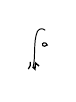
\begin{tikzpicture}[x=0.13cm,y=0.13cm,baseline=-0.5ex]
\draw[line width=0.35pt] (0,0) .. controls (0.3,1.1) and (0.0,2.6) .. (0.45,3.6) .. controls (0.65,3.9) and (0.95,3.9) .. (1.2,3.7);
\draw[line width=0.5pt] (0,0.1) -- (0.2,-0.1) -- (0.25,0.5) -- (0.6,0.2);
\draw[line width=0.4pt] (0.95,2.2) .. controls (0.8,2.5) and (1.3,2.6) .. (1.4,2.25) .. controls (1.2,2.1) and (1.05,2.1) .. (0.95,2.2);
\draw[line width=0.45pt] (-0.45,-0.1) .. controls (-0.25,0.1) and (-0.2,0.4) .. (-0.25,0.6);
\end{tikzpicture}}
On peut encore se demander si $\rho$ s'exprime en fonction des $\varepsilon_i$, et on trouve comme tantôt que non.

Quant à relever $\dot\tau$ en un élément de $\mathcal E$, par un chemin de $P$ à $\bar P$, on ne voit pas de choix privilégié --- on voit trois choix également naturels. Au lieu de les expliciter \unsure{direct$\bar m$t|directement}, je préfère considérer le sous-groupe d'isotropie de $P$ dans $\Gamma=\Gamma_{0\unsure{,|.}3}=\unsure{\mathfrak S_3|\mathcal S_3}\times\mathbb Z/2$, qui est formé des couples $\dot\sigma,\dot\tau^\varepsilon$ tels que $\operatorname{sg}(\dot\sigma)=\varepsilon$; \deleted{On} i.e. les éléments
\[
\widetilde{\dot\sigma}=(\dot\sigma,\dot\tau^{\operatorname{sg}(\dot\sigma)})\in\Gamma
\]
qui sont relevés canoniquement en des éléments $(\widetilde{\dot\sigma},\text{lacet trivial en }P)$ de $\mathcal E$. On trouve un hom
\[
(11)\quad\left\{\begin{aligned}
\underset{\unsure{:}}{\varphi}:\unsure{\mathfrak S_3|\mathcal S_3}&\longrightarrow\Gamma=\unsure{\mathfrak S_3|\mathcal S_3}\times\mathbb Z/2\\
\dot\sigma&\longmapsto\dot\sigma,\operatorname{sg}(\dot\sigma)
\end{aligned}\right.
\]
et un relèvement canonique de $\varphi$ en
\[
(12)\qquad\sigma\longrightarrow\tilde\sigma:\quad\unsure{\mathfrak S_3|\mathcal S_3}\longrightarrow\mathcal E
\]
On pose
\[
\tilde\sigma_i=\widetilde{\dot\sigma_i}
\]
\margin{on a d'autre part \deleted{$\unsure{\tilde\rho}$} $\widetilde{\dot\rho}=\rho$ 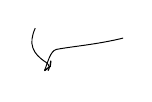
\begin{tikzpicture}[x=0.18cm,y=0.18cm,baseline=-0.5ex]
\draw[line width=0.35pt] (-0.5,2.8) .. controls (-1.0,1.7) and (-0.7,1.0) .. (0.25,0.4) .. controls (0.5,0.2) and (0.55,0.0) .. (0.4,-0.2);
\draw[line width=0.35pt] (5.7,2.1) .. controls (3.9,1.65) and (2.0,1.5) .. (1.0,1.3) .. controls (0.55,1.2) and (0.4,0.4) .. (0.15,-0.2);
\draw[line width=0.5pt] (0.15,-0.2) -- (0.55,0.1) -- (0.6,0.5);
\end{tikzpicture}}
\mspage{21}

\scanpage{23}
\mspage{10}
Le sous-groupe $\mathcal E_\tau$ de $\mathcal E$ image inverse de $\mathbb Z/2$ engendré par $\tau$, est le groupe cartographique ``triangulé pondéré'' de Malgoire, ayant comme gén $\tau_0,\tau_1,\tau_\infty$ \deleted{\unsure{relati.|relat.}} avec
\[
(17)\quad\left\{\begin{aligned}
\deleted{\unsure{\tau_1}\tau_\infty={}}\ l_0&=\tau_{\deleted{\unsure{0}}\infty}\tau_{\deleted{\unsure{\infty|0}}1}\\
\deleted{\tau_\infty\tau_0={}}\ l_1&=\tau_{\deleted{\unsure{\infty}}0}\tau_\infty\\
l_\infty&=\tau_1\tau_0
\end{aligned}\right.
\]
\margin{\uline{NB}\quad\begin{tikzpicture}[baseline=0.2ex]\draw (0,0.12)--(0.32,0.15);\fill (0.17,0.06) circle (0.015);\end{tikzpicture}}
$\mathcal E_\tau$ peut être considéré comme le groupe ayant comme \inserted{gén. les $\tau_i$, avec les} seules relations (16) --- on a un hom signature évident $\tau_i\longrightarrow-1$ de $\mathcal E_\tau$ dans $\pm1$, dont le noyau est $\Pi$ engendré par les $l_i$ décrits par (17)\ldots\ .

\figure{\begin{tikzpicture}\draw (0,0)--(0.8,0.025);\end{tikzpicture}}
\margin{\begin{tabular}{@{}l@{}}On a les\\relations\\[2ex]$\rho$\end{tabular}}
Revenons à une description plus symétrique des autom. extérieurs à lacets de $\mathcal E$. On désignera par $\hat{\mathcal E}$ le complété profini de $\mathcal E$, extension de $\hat\Gamma_{0,3}=\Gamma_{0,3}=\unsure{\mathfrak S_3|\mathcal S_3}\times\mathbb Z/2$ par $\hat\Pi$, et par $\widehat{\widehat{\mathcal E}}$ le groupe des autom. \deleted{\unsure{extérieurs}} \inserted{à} lacets de $\hat\Pi$, extension de $\widehat{\widehat\Gamma}=\operatorname{Aut}\operatorname{ext}_{\mathrm{lac}}(\hat\Pi)$ par $\hat\Pi$
\diagram{\begin{tikzcd}[column sep=large,row sep=small]
(18)\quad&1\arrow[r]&\hat\Pi\arrow[r]&\widehat{\widehat{\mathcal E}}\arrow[r]&\widehat{\widehat\Gamma}\arrow[r]&1\\
&&&&\unsure{\Vert|\cup}&\\
&&&&\operatorname{Aut}\operatorname{ext}_{\mathrm{lac}}(\hat\Pi)&
\end{tikzcd}}
\mspage{22}

\scanpage{24}
qui contient $\hat{\mathcal E}$ comme sous-extension. On désigne par $\mathord{\text{\begin{tikzpicture}[
  x=1em,y=1ex,baseline=0pt,
  line width=.045em,line cap=butt,line join=miter]
  \draw (.04,0)--(.04,1.60)--(.58,1.60)--(.58,1.40);
  \draw (.16,0)--(.16,1.40)--(.58,1.40);
\end{tikzpicture}}}$ le commutant de $\unsure{\mathfrak S_3|\mathcal S_3}$ dans $\widehat{\widehat\Gamma}$ \inserted{(\unsure{qui contient} $\dot\tau$)}, et par $\mathbb E$ l'extension correspondante de $\mathord{\text{\begin{tikzpicture}[
  x=1em,y=1ex,baseline=0pt,
  line width=.045em,line cap=butt,line join=miter]
  \draw (.04,0)--(.04,1.60)--(.58,1.60)--(.58,1.40);
  \draw (.16,0)--(.16,1.40)--(.58,1.40);
\end{tikzpicture}}}$ par $\hat\Pi$. Notons déjà que
\[
\left\{\begin{aligned}
\mathord{\text{\begin{tikzpicture}[
  x=1em,y=1ex,baseline=0pt,
  line width=.045em,line cap=butt,line join=miter]
  \draw (.04,0)--(.04,1.60)--(.58,1.60)--(.58,1.40);
  \draw (.16,0)--(.16,1.40)--(.58,1.40);
\end{tikzpicture}}}\cap\underset{\deleted{\unsure{\mathfrak S_3}}}{\unsure{\Gamma_{\unsure{0,3}}|\mathord{\text{\begin{tikzpicture}[
  x=1em,y=1ex,baseline=0pt,
  line width=.045em,line cap=butt,line join=miter]
  \draw (.04,0)--(.04,1.60)--(.58,1.60)--(.58,1.40);
  \draw (.16,0)--(.16,1.40)--(.58,1.40);
\end{tikzpicture}}}}}&=\{1,\tau\}\\
\mathord{\text{\begin{tikzpicture}[
  x=1em,y=1ex,baseline=0pt,
  line width=.045em,line cap=butt,line join=miter]
  \draw (.04,0)--(.04,1.60)--(.58,1.60)--(.58,1.40);
  \draw (.16,0)--(.16,1.40)--(.58,1.40);
\end{tikzpicture}}}\cap\unsure{\mathfrak S_3|\mathcal S_3}&=\{1\}
\end{aligned}\right.
\]
\margin{\deleted{\uline{\unsure{NB}}}}
\margin{\diagram{\begin{tikzcd}
&\unsure{\mathfrak S_3|\mathcal S_3}\times\widehat{\widehat\Gamma}^!\arrow[d,phantom,"{\cup}"]&&\\
\text{\uline{NB}}&\widehat{\widehat\Gamma}\arrow[r,phantom,"\supset"]&\underset{\deleted{\unsure{\Gamma}}}{\unsure{\mathfrak S_3|\mathcal S_3}}\times\mathord{\text{\begin{tikzpicture}[
  x=1em,y=1ex,baseline=0pt,
  line width=.045em,line cap=butt,line join=miter]
  \draw (.04,0)--(.04,1.60)--(.58,1.60)--(.58,1.40);
  \draw (.16,0)--(.16,1.40)--(.58,1.40);
\end{tikzpicture}}}&
\end{tikzcd}}
--- j'ignore si cette inclusion est une égalité, i.e. si $\mathord{\text{\begin{tikzpicture}[
  x=1em,y=1ex,baseline=0pt,
  line width=.045em,line cap=butt,line join=miter]
  \draw (.04,0)--(.04,1.60)--(.58,1.60)--(.58,1.40);
  \draw (.16,0)--(.16,1.40)--(.58,1.40);
\end{tikzpicture}}}\subset\widehat{\widehat\Gamma}^!$ est une égalité}
On veut donner d'abord une description plus symétrique des élts de $\widehat{\widehat{\mathcal E}}^!$, sans faire jouer un rôle particulier à $L_0$ engendré par $l_0$ $(L_0=\unsure{\hat k_0|\hat\kappa_0}(\hat{\mathbb Z}))$. Un $u\in\widehat{\widehat{\mathcal E}}$ est \inserted{pour être} défini par un multiplicateur
\[
(19)\qquad p=\chi(u)\in\hat{\mathbb Z}^{*}
\]
et des
\[
(20)\qquad g_i\in\hat\Pi\qquad i=0,1,\infty
\]
pour
\[
(21)\qquad u(l_i)=\operatorname{int}(g_i^{\unsure{\deleted{\unsure{-1}}|\unsure{-1}}})l_i^p
\]
les données (19), (20) étant liées par la relation
\[
(22)\qquad(\operatorname{int}(g_\infty^{\unsure{\deleted{\unsure{-1}}|\unsure{-1}}})l_\infty^p)
(\operatorname{int}g_1^{\unsure{\deleted{\unsure{-1}}|\unsure{-1}}}\cdot l_1^p)
(\operatorname{int}(g_0^{\unsure{\deleted{\unsure{-1}}|\unsure{-1}}})l_0^p)=1
\]
et par le fait que les $u(l_i)$ définis par (21) \uline{engendrent} $\hat\Pi$ \unsure{topolog\textsuperscript{t}|topologiquement}. Pour $u$ fixé, $p$
\mspage{23}

\scanpage{25}
\mspage{11}
est unique, et $g_i$ défini multiplication à gauche par un él. quelconque de $L_i$, soit $l_i^{\unsure{\alpha_i|\beta_i}}$ $(\alpha_i\in\hat{\mathbb Z})$. On passe de $u$ à $\operatorname{int}(g)\circ u$ en \inserted{gardant $p$, et en\unsure{,}} remplaçant les $g_i$ par les $gg_i$.

Si $v$ est donné par $q,(h_i)$, on a
\[
vu(l_i)=v(\operatorname{int}(g_i^{\unsure{\deleted{\unsure{-1}}|\unsure{-1}}})l_i^p)=\operatorname{int}(v(g_i^{\unsure{\deleted{\unsure{-1}}|\unsure{-1}}}))v(l_i)^p
\]
où
\[
v(l_i)=\operatorname{int}(h_i^{\unsure{\deleted{\unsure{-1}}|\unsure{-1}}})l_i^q\qquad\text{donc}\qquad v(l_i)^p=\operatorname{int}(h_i^{\unsure{\deleted{\unsure{-1}}|\unsure{-1}}})l_i^{pq}
\]
donc
\[
(23)\quad vu(l_i)=\operatorname{int}\bigl(\overset{\deleted{\unsure{(h_i v(g_i))^{-1}}}}{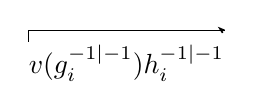
\begin{tikzpicture}[baseline=(prod.base)]
\node[inner sep=0pt] (prod) {$v(g_i^{\unsure{\deleted{\unsure{-1}}|\unsure{-1}}})h_i^{\unsure{\deleted{\unsure{-1}}|\unsure{-1}}}$};
\draw[line width=0.4pt] ([yshift=1pt]prod.north west) -- ([yshift=5pt]prod.north west) -- ([yshift=5pt]prod.north east);
\draw[line width=0.6pt] ([yshift=5pt]prod.north east) -- ++(-0.06,0.025) -- ++(0.035,-0.055);
\end{tikzpicture}}\bigr)l_i^{pq}
\]
Si on désigne par $S\overset{\unsure{\sim|\deleted{\sim}}}{\widehat{\widehat{\mathcal E}}}^!$ l'extension de $\widehat{\widehat{\mathcal E}}^!$ par $\hat{\mathbb Z}^{\{0,1,\infty\}}$ définie \deleted{\unsure{par le couple|par les couples|par le groupe}} \unsure{groupe|formé|formée} $\overset{\text{\begin{tikzpicture}[x=0.09cm,y=0.09cm,baseline=0ex]
\draw[line width=0.35pt] (0.45,0) .. controls (0.4,0.65) and (0.05,1.3) .. (0.02,1.05) .. controls (-0.05,0.65) and (0.5,0.35) .. (0.75,0.55) -- (1.15,1.1) -- (1.3,1.0);
\end{tikzpicture}}}{\text{des}}$\unsure{.} \deleted{couples} triples d'un $u\in\widehat{\widehat{\mathcal E}}^!$ et d'un système de $g_i$ qui explicitent \inserted{via (21)} l'isomorphisme de la structure à lacets ($p$ étant le multiplicateur), on a sur $S\overset{\unsure{\sim|\deleted{\sim}}}{\widehat{\widehat{\mathcal E}}}^!$ trois fonctions à valeurs dans $\deleted{\unsure{\mathcal E}}\hat\Pi$
\[
(u,(g_i))\overset{\gamma_i}{\longmapsto}g_i,
\]
et on aura\unsure{:}
\[
(24)\quad\gamma_i(\tilde v\tilde u)=\deleted{\unsure{\tilde v(\tilde u_i(\tilde u))\unsure{\cdot|:}\gamma_i(\tilde v)|\tilde v(\gamma_i(\tilde u))\unsure{\cdot|:}\gamma_i(\tilde v)}}\inserted{\deleted{\unsure{\gamma_i(\tilde v)\cdot v(\gamma_i(\tilde u))}} \tilde v(\gamma_i(\tilde u)\gamma_i\unsure{(}\tilde v)}
\]
i.e. $(\gamma_i)$ est un 1-cocycle sur le groupe \deleted{$\unsure{\widehat{\widehat{\mathcal E}}^!}$}\inserted{$S\overset{\unsure{\sim|\deleted{\sim}}}{\widehat{\widehat{\mathcal E}}}^!$} à valeurs dans le groupe \deleted{\unsure{produit du groupe}}\inserted{opposé au groupe} $\pi^{\{0,1,\infty\}}$.
\margin{\uline{NB} $S\widehat{\widehat{\mathcal E}}^!$ a été construit comme le groupe des Systèmes
\[
(p,g_0,g_1,g_\infty)\in\hat{\mathbb Z}^*\times\Pi^{[0,1,\infty]}
\]
satisfaisant la relation (22)}
\deleted{groupe}
Le sous-groupe de $S\widehat{\widehat{\mathcal E}}^!$ noyau de $S\overset{\unsure{\sim|\deleted{\sim}}}{\widehat{\widehat{\mathcal E}}}\longrightarrow\operatorname{Aut}\operatorname{ext}_{\mathrm{lac}}^!(\widehat{\unsure{\pi|\Pi}})$ s'identifie au groupe produit
\[
\left(\hat\Pi\times\prod_{i\in\{0,1,\infty\}}L_i\right)\simeq\widehat{\unsure{\pi|\Pi}}\times\underset{\begin{tikzpicture}[x=0.10cm,y=0.10cm,baseline=0ex]
\draw[line width=0.3pt] (0,1.35) -- (0.25,0) -- (0.65,1.25);
\draw[line width=0.3pt] (1.05,1.15) -- (1.15,0.1);
\fill (1.0,1.65) circle (0.08);
\end{tikzpicture}}{\unsure{(\hat{\mathbb Z})^{\{0,1,\infty\}}|(\hat{\mathbb Z})^3}}
\]
\mspage{24}

\scanpage{26}
en associant à $(g,(\unsure{\alpha^i|\alpha_i|\alpha'})_{i\in\{0,1,\infty\}})$ le système
\[
\deleted{\text{\unsure{de|des|dans}}}\quad p=1,\quad(g_\cdot)=\deleted{\unsure{(l_i^{\alpha_i})}}\deleted{\unsure{(l_i^{\alpha_i}g^{-1})|(l_i^{\alpha_i}g)}}(gl_i^{\alpha_i})
\]
Il faudrait expliciter les opérations des éléments $\sigma_i$ ou $\varepsilon_i$ \deleted{sur} $(\in S\overset{\unsure{\sim|\deleted{\sim}|\infty}}{\widehat{\widehat{\mathcal E}}}^{!})$ sur $\deleted{\unsure{u|\varepsilon}}\tilde u\in S\overset{\unsure{\sim|\deleted{\sim}|\infty}}{\widehat{\widehat{\mathcal E}}}^{!}$, par \deleted{\unsure{leurs|par la|de la}} conjugaison, et en particulier de $\rho$. On trouve que \deleted{$\unsure{p}$ (bien sûr)} les $\gamma_i$ sont ``covariants'' par $\rho$, i.e.
\[
\gamma_i(\rho\tilde u\rho^{-1})=\gamma_{i+1}\unsure{(}\bar u)
\]
\deleted{\unsure{i.e.|ici} \unsure{si} $\unsure{\hat u|\tilde u}$ est défini par}
\margin{\uline{NB} Il y a lieu d'introduire un groupe $S\hat{\mathcal E}$ extension de $\mathcal E$ par $\hat{\mathbb Z}^{\{0,1,\infty\}}$ (déduite d'une extension canonique de $\Gamma$ par $\mathbb Z^{\{0,1,\infty\}}$) et d'introduire \deleted{\unsure{des}} des relèvements des $\sigma_i,\rho$ par des éléments de $S\hat{\mathcal E}$\ldots\ .}
\mspage{25}

\scanpage{27}
\mspage{12}
L'extension $\mathcal E=\mathcal E_{0,3}$ de $\Gamma=\Gamma_{0,3}\simeq\underbrace{\unsure{\mathfrak S|\mathcal S}_{\unsure{[|\{}0,1,\infty]}}_{\unsure{=|\simeq}\unsure{\mathfrak S_3|\mathcal S_3}}\times\mathbb Z/2\mathbb Z$
\margin{engendré par $\tau:\ z\mapsto\bar z$}
par
\[
\Pi=\Pi_{0,3}=\{l_0,l_1,l_\infty\mid l_\infty l_1l_0=1\}=\Pi_1(\underbrace{\mathbb P^1_{\mathbb C}\setminus\{0,1,\infty\}}_{U=U_{0,3}},-\bar{\jmath}\}.
\]
Les classes de conjugaison \deleted{\unsure{au dessus des}} de scindages partiels maximaux correspondent aux points fixes de $\dot\rho,\dot\sigma_0,\dot\sigma_1,\dot\sigma_\infty$ opérant sur $X_{0,3}$, et \inserted{(éventuelles)} aux comp. connexes des ens. d'invariants de $\unsure{\deleted{\unsure{\dot\rho^2}}|{\unsure{\dot\rho|\rho}}^{\deleted{\unsure{2}}}}\tau,\dot\sigma_0\tau,\dot\sigma_1\tau,\dot\sigma_\infty\tau$. Les p\textsuperscript{ts} fixes de $\rho$ \inserted{\unsure{sont}} $P$ et $\bar P$ dont le stabilisateur est d'ordre $6$, \inserted{savoir $\varphi(\unsure{\mathfrak S_3|\mathcal S_3})$} formé de $1,\dot\rho,\dot\rho^2,\dot\sigma_1\tau,\dot\sigma_2\tau,\dot\sigma_3\tau$. On a étudié le relèvement correspondant \inserted{à $P$} (de $\varphi(\unsure{\mathfrak S_3|\mathcal S_3})$), on trouve des relèvements ($\Pi$-conjugués \inserted{entre eux}) relatifs à $\bar P$ s'obtiennent en \deleted{\unsure{conj}} prenant un élémt de $\mathcal E$ \deleted{\unsure{qui|et}} qui \unsure{soit|sont} au dessus d'un élémt de $\Gamma$ envoyant $P$ en $\bar P$ (savoir $\dot\sigma_0,\dot\sigma_{\unsure{1}},\dot\sigma_\infty,\tau,\tau\rho,\tau\rho^2$) et en conjuguant par cet élément on peut donc prendre \deleted{$\unsure{\sigma_0,\tau}$} un des éléments $\sigma_0,\sigma_1,\sigma_\infty$ (ou $\varepsilon_0,\varepsilon_1,\varepsilon_\infty$) ou $\tau_0,\tau_1,\tau_\infty$ ou \unsure{les|leurs} produits des précédents par \deleted{\unsure{ou|un|$\tau$}} $\rho$ ou $\rho^2$\ldots.

Le\deleted{\unsure{s}} \inserted{seul} p\textsuperscript{t\deleted{\unsure{s}}} fixe de $\sigma_0$ est $2$, dont le stabilisateur est le groupe $\simeq\mathbb Z/2\times\mathbb Z/2$ engendré par $\sigma_0$ et $\tau$. On a un relèvement de ce sous-groupe
\mspage{26}
